\documentclass[twocolumn]{aastex61}
\usepackage{bm}
\usepackage{color}
\usepackage{graphicx}

\newcommand\teff{T_{\rm eff}}
\newcommand\logg{\log{g}}
\newcommand\feh{[\rm{Fe}/\rm{H}]}

\newcommand{\project}[1]{\textsl{#1}}
\newcommand{\package}[1]{\texttt{#1}}
\newcommand{\acronym}[1]{{\small{#1}}}
\newcommand{\todo}[1]{\textcolor{red}{#1}}


\received{2018 XX XX}
\revised{2018 XX XX}
\accepted{2018 XX XX}

\graphicspath{figures/}

\submitjournal{AAS Journals}

\shorttitle{Short title}
\shortauthors{Hinkel et al.}

\begin{document}

\title{Long title}

\correspondingauthor{Natalie Hinkel}
\email{natalie.hinkel@gmail.com}

\author[0000-0003-0595-5132]{Natalie Hinkel}
\affiliation{Department of Physics \& Astronomy, 
			 Vanderbilt University, 
			 Nashville, TN 37235, USA}

\author[0000-0003-2866-9403]{David W. Hogg}
\affiliation{Center for Cosmology and Particle Physics, Department of Physics, 
			 New York University, 
			 726 Broadway, New York, NY 10003, USA}
\affiliation{Center for Data Science, 
			 New York University, 
			 60 Fifth Ave, New York, NY 10011, USA}
\affiliation{Max-Planck-Institut f\"ur Astronomie, 
			 K\"onigstuhl 17, D-69117 Heidelberg}
\affiliation{Flatiron Institute, 
			 162 Fifth Ave, New York, NY 10010, USA}

\author[0000-0003-0174-0564]{Andrew R. Casey}
\affiliation{School of Physics \& Astronomy, 
			 Monash University, 
			 Wellington Road, Clayton 3800, Victoria, Australia}
\affiliation{Faculty of Information Technology, 
			 Monash University, 
			 Wellington Road, Clayton 3800, Victoria, Australia}


\begin{abstract}
Abstract.
\end{abstract}


\keywords{}

\section{Introduction}
\label{sec:introduction}


\section{Methods}
\label{sec:methods}




\begin{figure}
	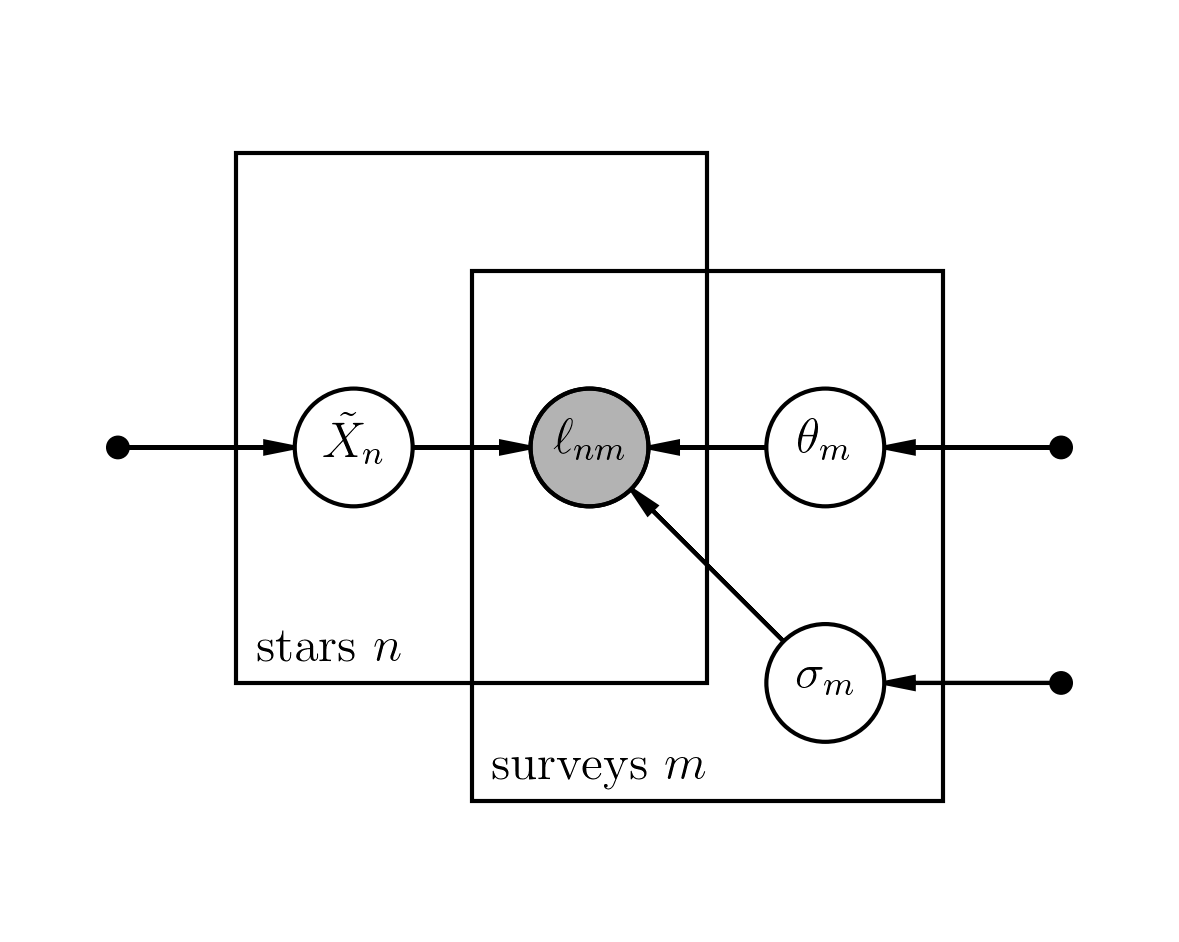
\includegraphics[width=0.5\textwidth]{figures/pgm.png}
    \caption{Probabilistic graphical model.}
\end{figure}


\acknowledgements

It is a pleasure to thank
	Dan Foreman-Mackey
for useful conversations.
This work was partly supported through the Australian Research Council 
through Discovery Grant DP160100637.


\software{
	\package{Astropy} \citep{astropy},
    \package{IPython} \citep{ipython},
    \package{matplotlib} \citep{mpl},
    \package{numpy} \citep{numpy},
    \package{scipy} \citep{scipy},
    \package{Stan} \citep{stan},
    \package{Daft} % http://daft-pgm.org/
    %tensorflow
}    

\bibliographystyle{aasjournal}
\bibliography{uberchemical}



\end{document}
